Twelve congruent disks are placed on a circle $C$ of radius 1 in such a way that the twelve disks cover $C$, no two of the disks overlap, and so that each of the twelve disks is tangent to its two neighbors. The resulting arrangement of disks is shown in the figure below.  The sum of the areas of the twelve disks can be written in the from $\pi(a-b\sqrt{c})$, where $a,b,c$ are positive integers and $c$ is not divisible by the square of any prime. Find $a+b+c$.

\begin{center}
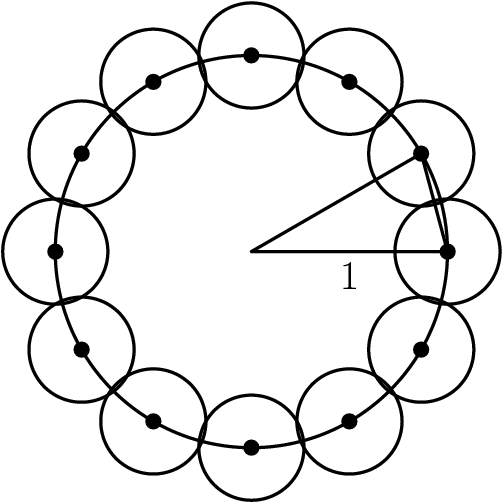
\includegraphics[width = 50.400000000000006mm]{img/fig0.png}
\end{center}